
\blank
\newpage

\section{Common LLM Architectures}

    I modelli linguistici di grandi dimensioni (LLM) possono essere classificati in base al loro scopo e alla loro architettura:

    \begin{itemize}
        \item \textbf{Embedding LLM e Generator LLM}: I primi, tipicamente \textit{Encoder-only}, generano rappresentazioni vettoriali del testo in input. I secondi, di tipo \textit{Decoder-only}, generano testo in linguaggio naturale a partire da un prompt.
        \item \textbf{Foundational e Instruction-tuned}: I modelli fondazionali (o di base) sono general-purpose e vengono addestrati su enormi quantità di dati con tecniche \textit{self-supervised} per catturare la conoscenza linguistica. I modelli instruction-tuned vengono invece addestrati su dataset annotati, tramite tecniche supervisionate (Supervised Fine Tuning - SFT), per seguire specifiche istruzioni fornite in input.
        \item \textbf{Multilingual e Multimodal}: Esistono modelli capaci di operare su più lingue e modelli multimodali che possono ricevere in input non solo testo, ma anche immagini, video e audio.
    \end{itemize}

    \subsection{Architettura Mixture of Experts (MoE)}

        L'aumento della dimensione di un modello garantisce in genere prestazioni migliori, ma richiede un budget di calcolo elevato. Un'architettura \textit{Mixture of Experts} (MoE) rappresenta un compromesso: permette di pre-addestrare modelli aumentandone drasticamente i parametri senza incrementare il budget di calcolo rispetto a un modello denso. 

        \begin{figure}[H]
            \centering
            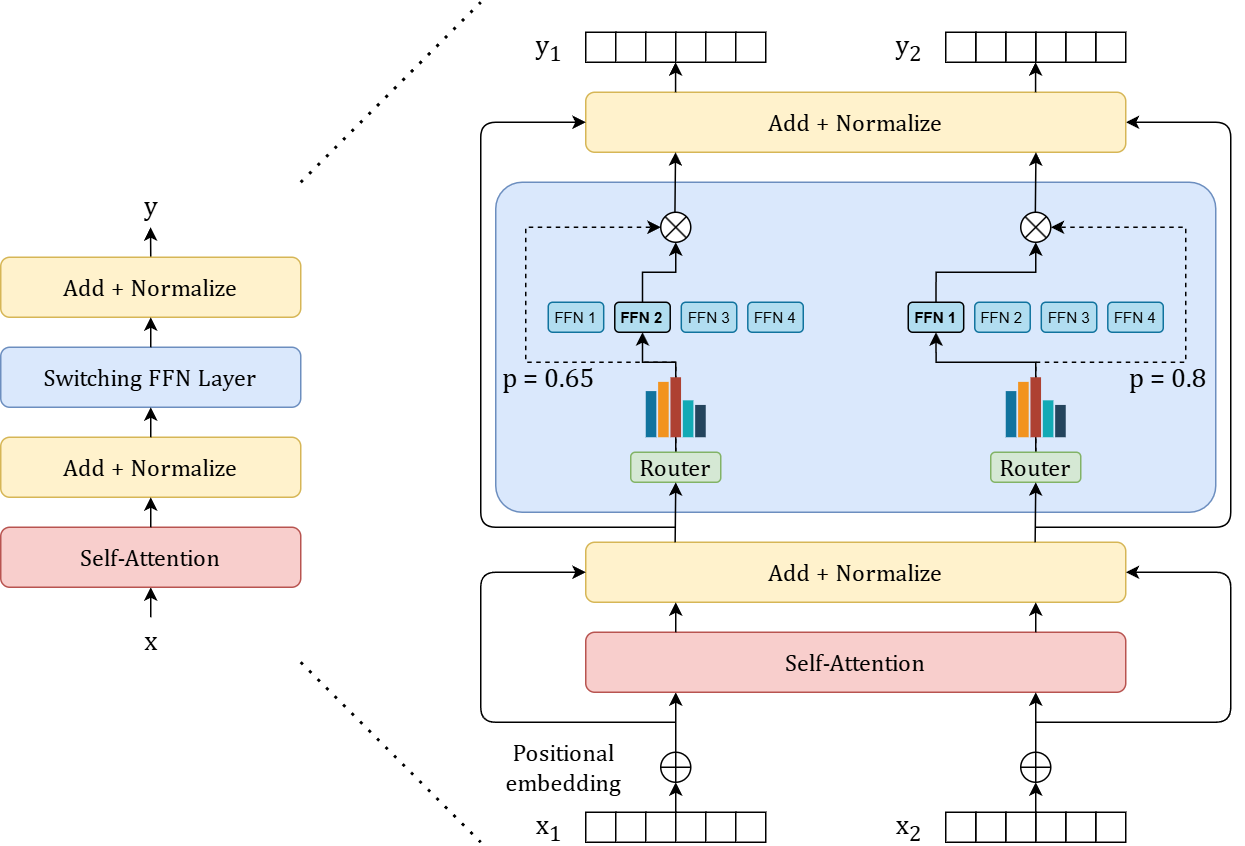
\includegraphics[width=0.7\linewidth]{imgs/schema_9_1.png}
            \label{fig:fig91}
        \end{figure}

        Un modello MoE si compone di due elementi chiave:
        
        \begin{enumerate}
            \item \textbf{Esperti (Layer MoE sparsi)}: Sostituiscono i tradizionali layer densi Feed-Forward Network (FFN). Ogni esperto è una rete neurale specializzata (su specifici gruppi di token o concetti, come la punteggiatura o i nomi propri).
            \item \textbf{Gate Network (Router)}: Determina a quali esperti inviare ciascun token. Il router ha parametri apprendibili e viene pre-addestrato insieme al resto della rete.
        \end{enumerate}

        Nonostante i MoE siano molto efficienti nel pre-training e consentano un'inferenza più rapida rispetto ai modelli densi (poiché solo una frazione dei parametri viene attivata), storicamente soffrono di overfitting durante il fine-tuning e presentano requisiti di memoria RAM elevati, dato che tutti i parametri devono essere caricati.

    \newpage

    \begin{figure}[H]
        \centering
        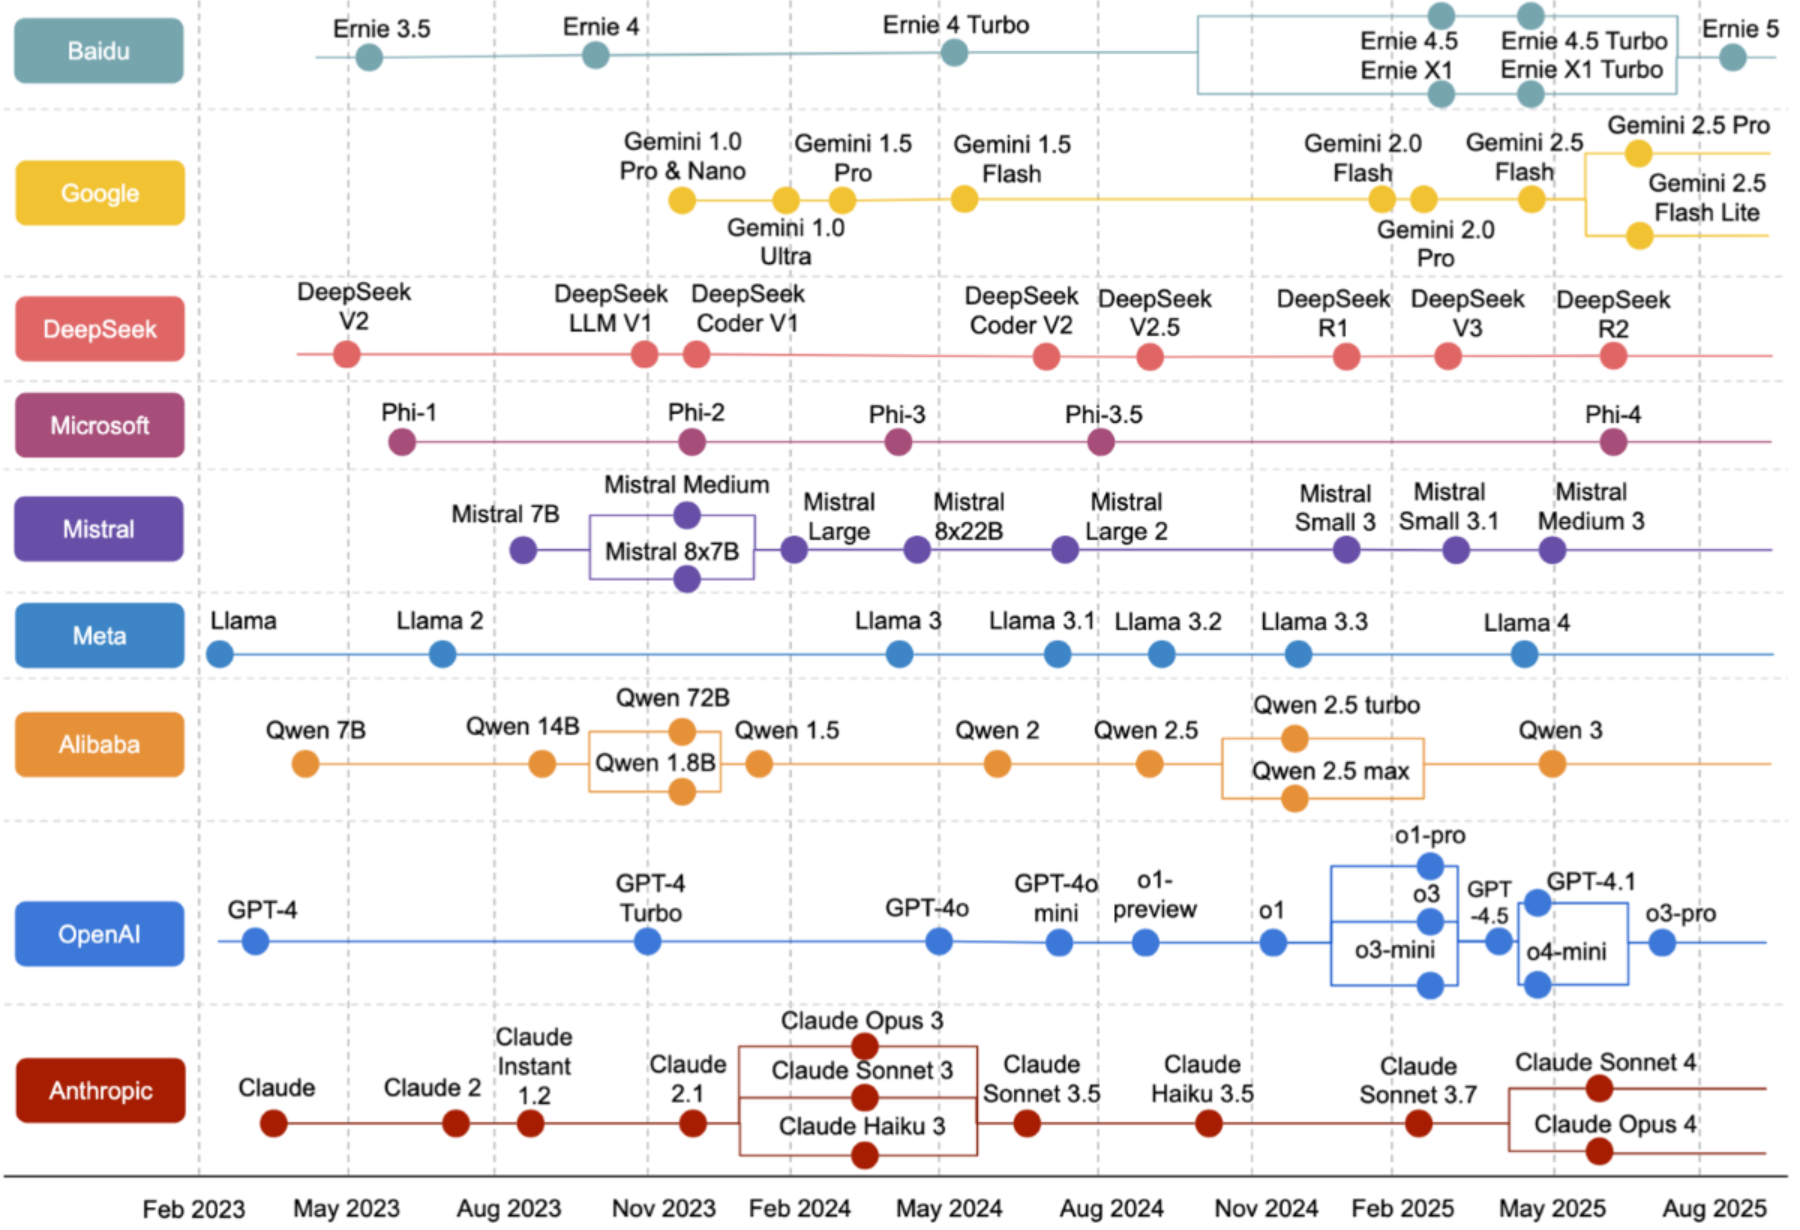
\includegraphics[width=1\linewidth]{imgs/schema_9_2.png}
        \label{fig:fig92}
    \end{figure}

    \newpage

    \subsection{La Famiglia GPT}      

        La famiglia Generative Pre-trained Transformer (GPT), sviluppata da OpenAI, si basa su architetture \textit{decoder-only} sottoposte a pre-training per il Language Modeling e successivo fine-tuning supervisionato. Il modello GPT originale utilizza uno stack di 12 blocchi transformer decoder e adotta la funzione di attivazione GeLU al termine di ogni blocco FFN.

        \begin{figure}[H]
            \centering
            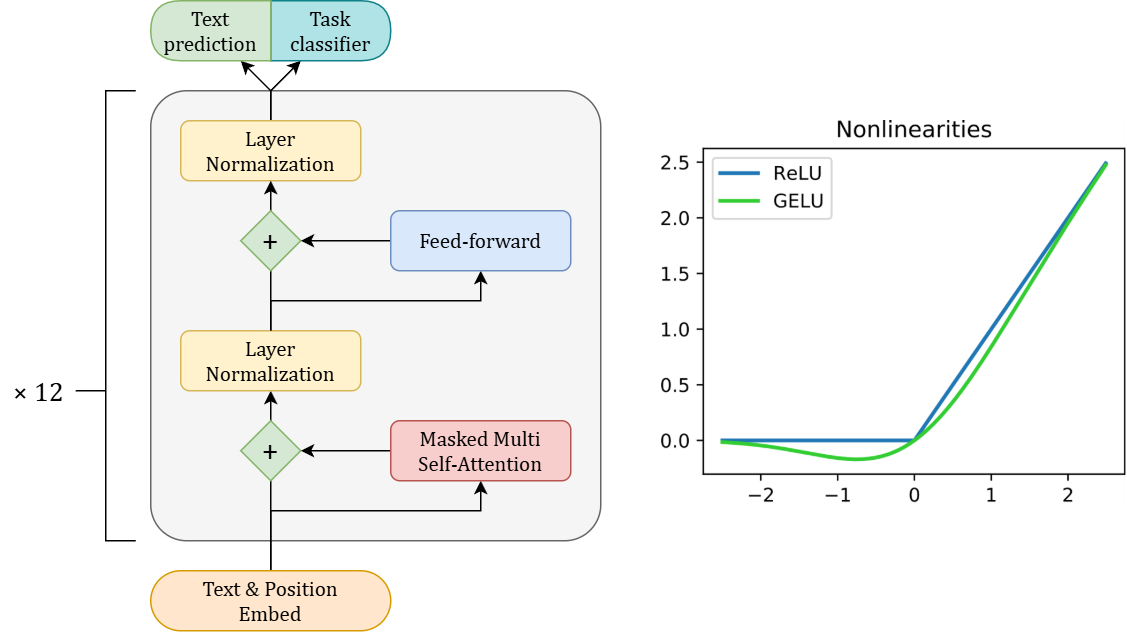
\includegraphics[width=0.7\linewidth]{imgs/schema_9_3.png}
            \label{fig:fig93}
        \end{figure}

        La funzione GeLU (Gaussian Error Linear Unit) modula l'attivazione lineare tramite la distribuzione cumulativa gaussiana ed è approssimata dalla seguente formula:
        $GELU(x) \sim x\sigma(1.702x)$

        \subsubsection{Pre-training e Fine-tuning in GPT}
    
            \begin{wrapfigure}{r}{0.5\textwidth}
                \vspace{-15pt}
                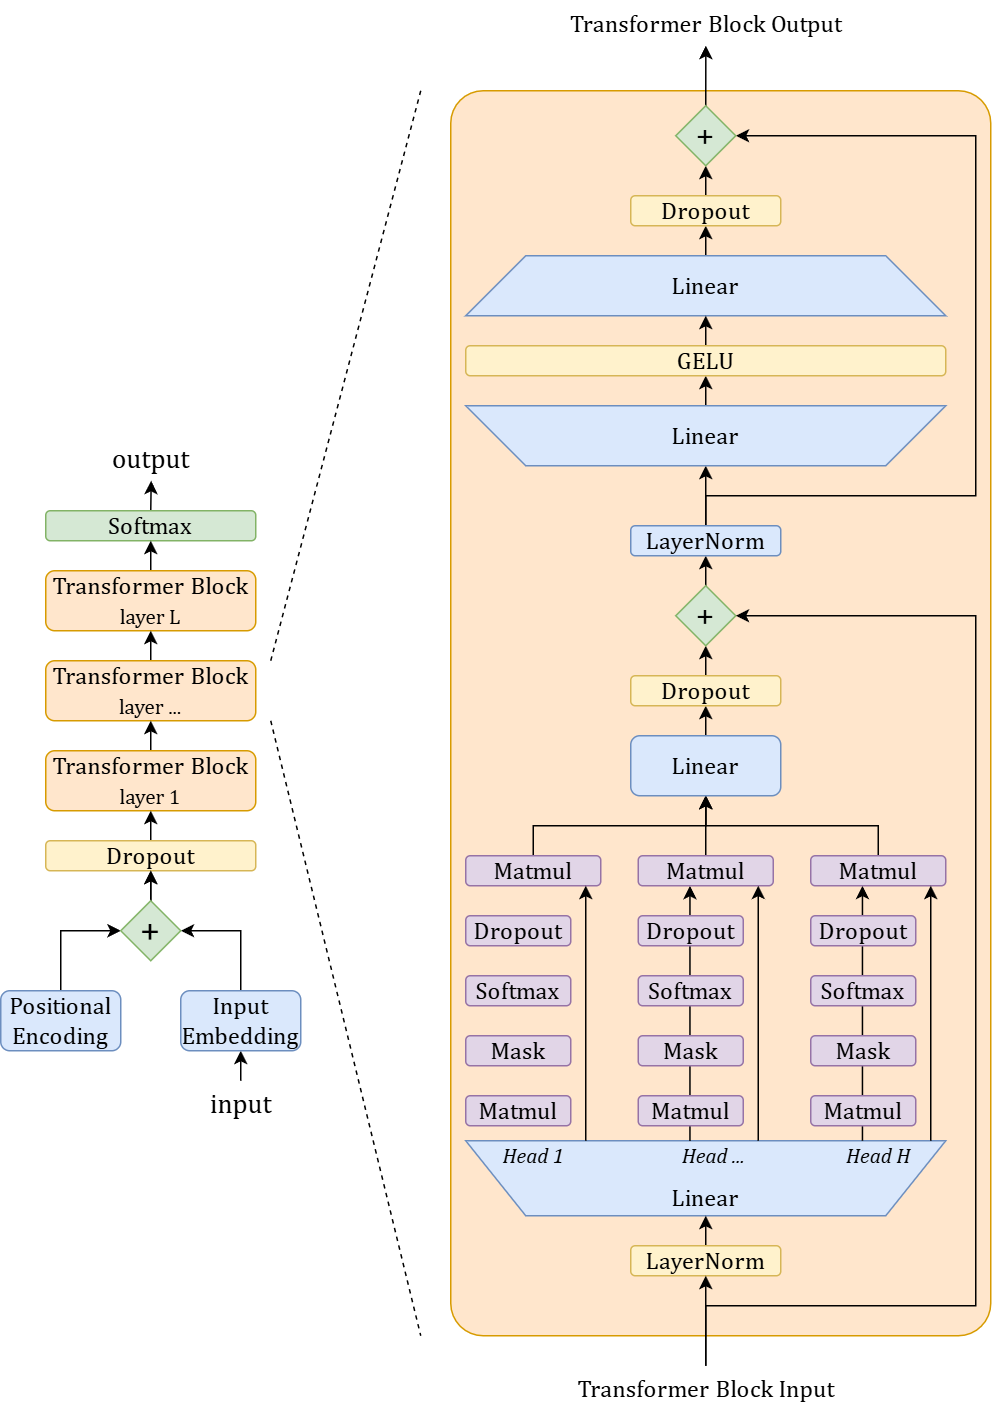
\includegraphics[width=1\linewidth]{imgs/schema_9_4.png}
                \label{fig:fig94}
            \end{wrapfigure}
            
            Durante il pre-training non supervisionato, dato un insieme di token $U=\{u_1,...,u_n\}$, il modello calcola la probabilità attraverso le seguenti trasformazioni, partendo dagli embedding testuali e posizionali:
            
            \begin{itemize}
                \item $h_0 = UW_e + W_p$
                \item $h_i = transformer\_block(h_{i-1}) \forall i \in [1,n]$
                \item $P(u) = softmax(h_n W_e^T)$
            \end{itemize}

            La funzione di loss per il pre-training massimizza la predizione del token successivo:
            $$L_1(\mathcal{U}) = \sum_i \log P(u_i|u_{i-k},...,u_{i-1};\Theta)$$

            Nel fine-tuning supervisionato, viene aggiunto un layer lineare finale per predire un'etichetta $y$ da una sequenza $x^1,...,x^m$:
            $$P(y|x^1,...,x^m) = softmax(h_l^m W_y)$$

            La funzione obiettivo finale combina la loss del pre-training e quella del fine-tuning:
            $$L_3(\mathcal{C}) = L_2(\mathcal{C}) + \lambda * L_1(\mathcal{C})$$

    \clearpage
    \newpage

    \subsection{Architetture Ottimizzate: LLaMA e Mistral}

        Modelli più recenti hanno introdotto varianti architetturali per migliorare stabilità e prestazioni. 

        \subsubsection{LLaMA (Meta)}

            La serie LLaMA utilizza una versione modificata dell'architettura transformer decoder-only con alcune differenze chiave rispetto a GPT:
            
            \begin{itemize}
                \item \textbf{SwiGLU}: Sostituisce la ReLU. Combina le funzioni Swish e Gated Linear Unit. La formulazione integra le attivazioni:
                $$SwiGLU(x) = x \cdot \sigma(\beta x) + (1 - \sigma(\beta x)) \cdot \sigma(W \cdot x + b)$$
                \item \textbf{Rotary Positional Embedding (ROPE)}: Codifica la posizione relativa tra i vettori di self-attention direttamente attraverso matrici di rotazione. Per i vettori query e key, la relazione diventa:
                $$q_m^\top k_n = x_m^\top W_q^\top R_{\theta,n-m} W_k x_n$$
                \item \textbf{RMSNorm}: Sostituisce la LayerNorm classica per ridurre il carico computazionale e stabilizzare il training. La formula è:
                $$\hat{x} = \frac{x}{RMS(x) + \epsilon}$$
            \end{itemize}

        \subsubsection{Mistral}

            I modelli Mistral introducono tecniche avanzate di gestione dell'attention per migliorare il throughput e la velocità:
            
            \begin{itemize}
                \item \textbf{Grouped-Query Attention (GQA)}: Le \textit{head} delle query sono divise in gruppi, e ciascun gruppo condivide una singola \textit{head} per chiavi (keys) e valori (values), riducendo la memoria richiesta durante il decoding.
                \item \textbf{Sliding Window Attention (SWA)}: Consente di gestire sequenze di contesto più lunghe riducendo i costi computazionali attraverso finestre di attenzione fisse.
            \end{itemize}

    \subsection{Altri Modelli e Approcci}

        \begin{itemize}
            \item \textbf{Claude (Anthropic)}: Focus sull'allineamento tramite \textit{Constitutional AI} e RLHF, per garantire risposte etiche e sicure basate su principi guida predefiniti.
            \item \textbf{Gemini e Gemma (Google)}: Gemini sfrutta MoE multimodali e Multi-Query Attention (MQA). Gemma è una versione open-source "distillata" (Knowledge Distillation) da Gemini, disponibile in versioni pre-addestrate (PT) e instruction-tuned (IT).
            \item \textbf{DeepSeek}: Implementa la \textit{Multi-head Latent Attention (MLA)}, che utilizza un'approssimazione a basso rango per comprimere lo spazio della cache Key-Value (KV), risultando estremamente efficiente in fase di inferenza.
        \end{itemize}
